\documentclass[10pt,twocolumn]{witseiepaper}

\usepackage{KJN}

\ifpdf
\pdfinfo{
/Title (ELEN4012 - Feature Based Automatic Modulation Classification)
/Author (Jacques Visser and Anthony Farquharson)
}
\fi

\begin{document}

\title{ELEN4012 - Feature Based Automatic Modulation Classification}

\author{Jacques Visser and Anthony Farquharson
\thanks{School of Electrical \& Information Engineering, University of the
Witwatersrand, Private Bag 3, 2050, Johannesburg, South Africa}
}

% TODO Rewrite abstract once the rest of the contents are figured out.
\abstract{Automatic modulation classification involves identifying the modulation scheme used in a signal without the decision being guided by an operator. This report covers a preliminary investigation into the design and implementation of such a system. An overview of the relevant literature is presented and proposals are made regarding the details of the implementation and testing of such a system using and Ettus USRP.}

\keywords{modulation, classification, USRP, UHD}

\maketitle
\thispagestyle{empty}\pagestyle{empty}

% TODO How does one even write an introduction?
\section{INTRODUCTION}

\section{LITERATURE SURVEY}
Zhu and Nandi \cite{zhu2014automatic} identifies three major approaches to automatic modulation classification; likelihood-based, distribution-test-based and feature-based. These are briefly detailled below.
	\subsection{Likelihood Based Classification}
	\subsection{Distribution Test Based Classification}
	\subsection{Feature Based Classification}
	\label{sec:features}
	Feature based AMR has been shown to be non-ideal, but significantly less computationally intensive \cite{zhu2014automatic} than the aforementioned methods.

	There are again three major approaches to feature-based AMC. These make use features derived from either the signal spectrum, the wavelet transform of the signal or high-order statistical representations of the signal \cite{zhu2014automatic}. 
	
	The classification of analog modulation schemes using spectral features is well documented by Zhu and Nandi \cite{zhu2014automatic} as well as Azzouz and Nandi \cite{azzouz2013automatic}. They make use of nine features, which are as follows:

	\begin{enumerate}
		\item $\gamma_{max}$: Maximum value of Power Spectral Density 
		\item $\sigma_{ap}$: Standard deviation of the absolute value of the non-linear component of the instantaneous phase.
		\item $\sigma_{dp}$: Standard deviation of the non-linear component of the direct instantaenous phase.
		\item $P$: Spectrum symmetry
		\item $\sigma_{aa}$: Standard deviation of the absolute value of the normalized and centered instantaneous amplitude
		\item $\sigma_{af}$: Standard deviation of the absolute value of the normalized and centered instantaneous frequency
		\item $\sigma_{a}$: Standard deviation of the normalized and centered instantaneous amplitude
		\item $\mu_{42}^{a}$: Kurtosis of the normalized and centered instantaneous amplitude
		\item $\mu_{42}^{f}$: Kurtosis of the normalized and centered instantaneous frequency
	\end{enumerate}
	

\section{EXISTING SOLUTIONS AND APPLICATIONS OF AMC}
	\subsection{Military}
		% jamming, listening in on communications
	\subsection{Civilian}
		% cognative radio, effective use of bandwith
		% aircraft monitoring

\section{SOLUTION SELECTION}

\section{DESIGN PROCESS OVERVIEW}
	\subsection{Development Methodology}
		% Engineering oriented method
		% make use of Trello
		% Add screenshots to appendix
	\subsection{Estimated Project Schedule}
		% Design, Implementation, Simulated Testing, Iteration, Practical Testing and Evaluation
		% Overview and Trello screenshots
	\subsection{Estimated Costs and Hardware Required}
		The practical implementation of this project will require at least two USRP devices. The first of which will be used for receiving radio signals, the modulation of which is to be classified. The second will be used to generate modulated signals in order to practically test the operation of the system. Seeing as Wits has these available, no charges would be incurred.

		Furthermore, at least two computers running Linux will be required. The team-members' labptops will be used for this purpose.

\section{IMPLEMENTATION OVERVIEW}
	\subsection{Hardware}
		% USRP
		% Antenna?
		% Runs on a Linux pc, not win cos of UHD
	As mentioned before, two USRP's and two computers are neccesary. To avoid significant effort in compiling and installation of the USRP Hardware Driver (UHD) both computers will run Linux natively.

	\subsection{Software}
		\subsubsection{Basic Software Structure}
			Due to the computationally intensive and time-dependent nature of the system, the software would have to be threaded, with each major component running on it's own thread.

			The software would consist of various components centered around a main control loop. The UHD driver, run in it's own thread, passes the signal to the central control stucture, which filters the signal and passes it to various feature extraction functions, all run in parralel. These functions deliver the features that have been extracted form the signal to a classifier which finally determines the modulation scheme used. This process is represented as a flow diagram in Figure \ref{fig:sw_overview}
			% fundamentally threaded
			% UHD on one thread
			% each of the feature extraction functions on their own thread
			% classifier on a final thread
		\subsubsection{Libraries and API's}
			Due to the complicated nature of the software implementation, all of the components will not be locally developed. Rather, various API's and libraries will be used.

			Firstly, the Ettus USRP Hardware Driver's (UHD) C++ API will be used for communication with the USRP. This is a free \& open source piece of software released under the GPLv3 license \cite{uhd_license}, and is thus free to be used for a project such as this.

			In order to spectrally analyse the incoming signal the KissFFT library is to be used. KissFFT is developed by Mark Borgerding and is available under a Revised BSD license \cite{kissfft_license}

			For displaying graphical information SFML (Simple and Fast Multimedia Library) will be used. This is distributed under the zlib/libpng License and may thus be freely used in a project such as this \cite{sfml_license}.

			For threading and other miscelaneous functions the C++ 11 Standard library will be used. GNU libstdc++ which is used with GCC is distributed under the GPLv3 license.

		\subsubsection{Build System}
			Due to the open-source nature and wide availability of the libraries and API's used in this project the software produced will be able to run on various platforms. To fully support this the CMake build-system-generator will be used so that this project may easily be compiled on various platforms.

			CMake is distributed under the BSD 3-Clause license \cite{cmake_license} and it can thus be distributed with and used in this project.
			% Cmake because easy, also can be compiled on windows (probably UHD issue, though)

		\subsection{Feature Extraction Functions}
			Individual functions will have to be developed for the extraction of each of the nine features mentioned in section \ref{sec:features}. Some of these features incorporate common data, thus the process of feature extraction may be accelerated by doing the computation thereof only once.

			A spectral representation of the signal is used in the process of obtaining most of the features. This is computed with an FFT using the KissFFT library. 
			
			To obtain the instantaneous phase of the signal, the negative portion of the spectral representation of the signal is to be removed and an IFFT is to be performed \cite{picinbono1997instantaneous}. Following this, phase unwrapping must be performed \cite{park2009introduction, picinbono1997instantaneous}.

			The Instantaneous frequency of the signal may then be obtained from the instantaneous phase by differentiation \cite{park2009introduction}.

			This results in a complex series of events. They are shown in sequence as a flow diagram in Figure \ref{fig:feature_flow}.

		\subsection{Signal Filtering}
			Filtering of the input signal to isolate the bandwidth in which a single signal exists is a delicate process. 
			Phase distortion may negatively affect the results as some of the features are dependant on the non-linear portion of the phase only. 
			Thus it is important to implement zero-phase digital filtering.
			This may be done by either performing forward and reverse filtering or by selecting an FIR filter with a vary flat phase response \cite{something?}.

			The former option would require buffering a large portion of the signal, but might yeild better results than the latter. This tradeoff, as well as selecting the bandwith of the band-pass filter to be used is still under investigation.

		\subsection{Classifier}


\section{PROPOSED TESTING PROCEDURE}
	\subsection{Simulated Testing}
		% Evaluate system with generated signals
		% See how well it fares with different number of samples
		% Signal to noise ratio
	\subsection{Practical Testing}
		% correlate real world results with simulation
		% Don't make a new program, just use GNURadio companion to make signals to classify

\section{PRELIMINARY RESULTS}
	Simple testing of the feature-based AMC algorithm was performed in MATLAB with a limited number of features. The results are promising, showing a clear seperation between different modulation schemes. This can be seen in Figure \ref{fig:plot0}. 

	The marked clustering of the results show that it is indeed possible to make use of a simple threshold-based decision-tree classifier. Making use of such a classifier, however, would require intense interaction with the application to set the appropriate thresholds. Thus it has been deemed appropriate to make use of a K-Nearest-Neighbor clustering algorithm so as to maximise the application's autonomy and extensibility.

	\begin{figure*}[!h]
		\centering
		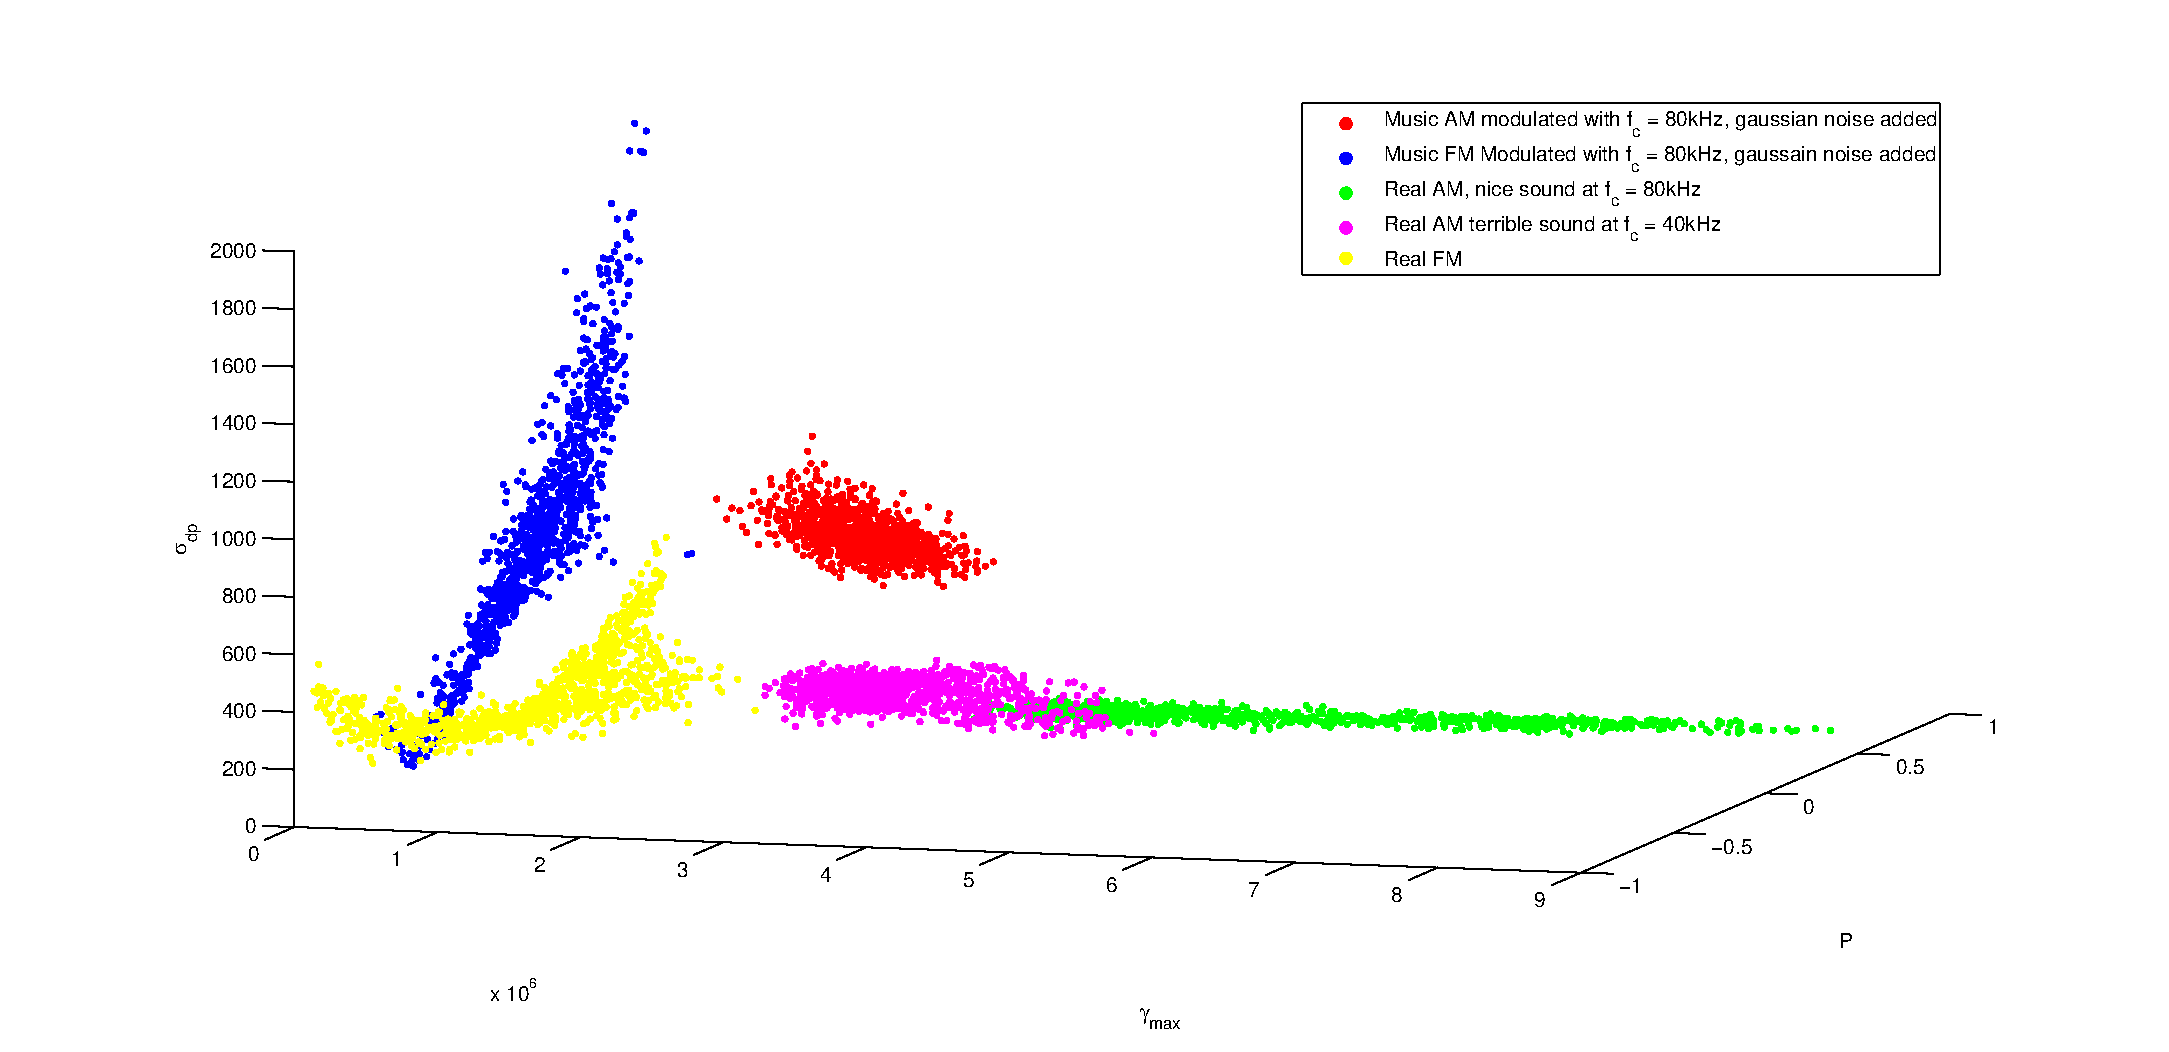
\includegraphics[width=1.1\textwidth]{plot0.eps}
		\caption{Plot of $\sigma_{dp}$ vs. $\gamma_{max}$ vs. $P$ for various AM and FM signals}
		\label{fig:plot0}
	\end{figure*}

\section{CONCLUSION AND RECOMMENDATIONS}


\bibliographystyle{witseie}
\bibliography{prelim} 
\end{document}
